\documentclass{article}
\usepackage[utf8]{inputenc}
\usepackage{graphicx}
\usepackage{amsmath}
\usepackage{amsfonts}
\usepackage{float}
\usepackage[a4paper, margin=1in]{geometry}
\title{Homework 8}
\author{Steve Gillet}
\date{\today}

% Custom information
\newcommand{\className}{Course: Algorithmic Motion Planning – ASEN 5254-001 – Fall 2024}
\newcommand{\professorName}{Professor: Morteza Lahijanian}
\newcommand{\taName}{Teaching Assistant: Yusif Razzaq}

\begin{document}

% Title
\maketitle
\begin{center}
    \large{\className} \\
    \large{\professorName} \\
    \large{\taName}
\end{center}

\section*{Exercise 1.
Extend your implementation of the GoalBiasRRT planner in \textit{Homework 7} to plan for \( m \) disk robots translating and rotating in a workspace \( W \subset \mathbb{R}^2 \) using a coupled (centralized) approach. Every robot \( A^i \) for all \( i \in \{1, \dots, m\} \) is a disk with radius \( R \). The initial position of robot \( i \) (center of disk) is at \( x_{\text{start}}^i \), and its goal is (center of disk) \( x_{\text{goal}}^i \). Further assume that all \( m \) robots move at the same speed. That is, 1 step for robot \( A^i \) is equal to 1 step for robot \( A^j \) for all \( i, j \in \{1, \dots, m\} \).
Your planner should take as input a step size \( r \), a goal bias probability \( p_{\text{goal}} \), maximum number of iterations \( n \), workspace obstacles, workspace boundaries, \( m \) robots and their corresponding initial position \( x_{\text{start}}^i \) and goal position \( x_{\text{goal}}^i \), and radius \( \epsilon \) (centered at \( x_{\text{goal}}^i \)) for the termination condition at goal as input and return a valid path for every robot from \( x_{\text{start}}^i \) to \( x_{\text{goal}}^i \), the size of the RRT tree, and the computation time.
\begin{itemize}
    \item Consider a 2D rectangular workspace \( W = [0, 16] \times [0, 16] \), with obstacle space \( W O \subset W \). Let \( W O = \bigcup_{i=1}^6 W O_i \), where each \( W O_i \) is a rectangle in \( W \) with the following vertices:
    \[
    \begin{aligned}
        W O_1: & \quad v_1^1 = (4, 6), \quad v_2^1 = (6, 6), \quad v_3^1 = (6, 7), \quad v_4^1 = (4, 7) \\
        W O_2: & \quad v_1^2 = (4, 6), \quad v_2^2 = (5, 6), \quad v_3^2 = (5, 10), \quad v_4^2 = (4, 10) \\
        W O_3: & \quad v_1^3 = (4, 9), \quad v_2^3 = (6, 9), \quad v_3^3 = (6, 10), \quad v_4^3 = (4, 10) \\
        W O_4: & \quad v_1^4 = (10, 6), \quad v_2^4 = (12, 6), \quad v_3^4 = (12, 7), \quad v_4^4 = (10, 7) \\
        W O_5: & \quad v_1^5 = (11, 6), \quad v_2^5 = (12, 6), \quad v_3^5 = (12, 10), \quad v_4^5 = (11, 10) \\
        W O_6: & \quad v_1^6 = (10, 9), \quad v_2^6 = (12, 9), \quad v_3^6 = (12, 10), \quad v_4^6 = (10, 10)
    \end{aligned}
    \]
    \item Consider a set of \( m = 6 \) disk robots, where \( R = 0.5 \) with the following start and goal configurations:
    \[
    \begin{aligned}
        x_{\text{start}}^1 &= (2, 2), \quad x_{\text{goal}}^1 = (14, 14) \\
        x_{\text{start}}^2 &= (2, 14), \quad x_{\text{goal}}^2 = (14, 2) \\
        x_{\text{start}}^3 &= (8, 14), \quad x_{\text{goal}}^3 = (8, 2) \\
        x_{\text{start}}^4 &= (2, 8), \quad x_{\text{goal}}^4 = (14, 8) \\
        x_{\text{start}}^5 &= (11, 2), \quad x_{\text{goal}}^5 = (5, 14) \\
        x_{\text{start}}^6 &= (11, 14), \quad x_{\text{goal}}^6 = (5, 2)
    \end{aligned}
    \]
\end{itemize}
}

\subsection*{(a) Answer the following questions:}

\subsubsection*{i. What is the C-space of each individual disk robot?}

The C-space (configuration space) of each individual disk robot is a two-dimensional space \( \mathbb{R}^2 \), representing the possible \(x\) and \(y\) positions of the robot in the workspace.

\subsubsection*{ii. What is the C-space of the meta-agent (composed space)?}

The C-space of the meta-agent, which combines the configuration spaces of all individual agents, is the Cartesian product of each robot's C-space. For \(m\) robots, this becomes \( \mathbb{R}^{2m} \), where each pair of dimensions represents the \(x\) and \(y\) coordinates of each robot.

\subsubsection*{iii. Describe how the C-space grows with respect to the number of agents.}

The C-space grows linearly with the number of agents in terms of dimensionality. For each additional robot, two more dimensions are added to the configuration space. So, for \(m\) robots, the dimension of the C-space is \(2m\).

\subsubsection*{iv. Is the growth rate a concern for scaling to larger numbers of agents? Justify your answer.}

Yes, the growth rate is a concern because the increased dimensionality makes the space exponentially harder to search for feasible paths. As the number of agents increases, the complexity of collision checking and path planning in higher-dimensional spaces grows significantly, which can impact computational efficiency and feasibility.

\subsection*{(b) Solve planning problem for \(m = 2\) using the first two robots (\(i = \{1, 2\}\)).
Let \( n = 7,500 \), \( r = 0.5 \), \( p_{\text{goal}} = 0.05 \), and \( \epsilon = 0.25 \). Plot the solution in the workspace showing \textbf{both} agents reaching their respective goals.
}

\begin{figure}[H]
    \centering
    \includegraphics[width=0.7\textwidth]{partBPlot.png} 
    \caption{Solution plot for \(m = 2\) with agents reaching their respective goals.}
    \label{fig:partBPlot}
\end{figure}

\subsection*{(c) Use 100 runs to benchmark your implementation in two categories:
\begin{itemize}
    \item \textbf{Computation time:} Measure the time taken for each run.
    \item \textbf{Size of the tree:} Record the number of nodes in the RRT tree.
\end{itemize}
Show your results using boxplots. Additionally, save the data in a format suitable for later analysis.
}

\begin{figure}[H]
    \centering
    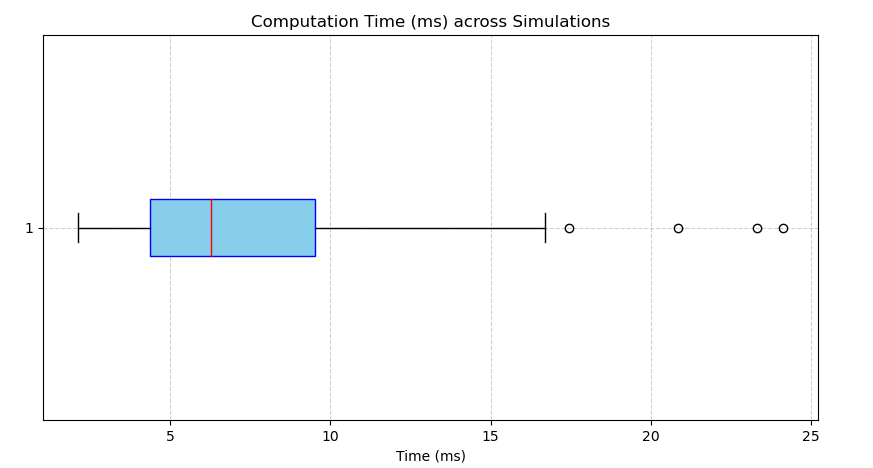
\includegraphics[width=0.7\textwidth]{1c2time.png} 
    \caption{Box plot for \(m = 2\) times over 100 iterations.}
    \label{fig:ic2time}
\end{figure}

\begin{figure}[H]
    \centering
    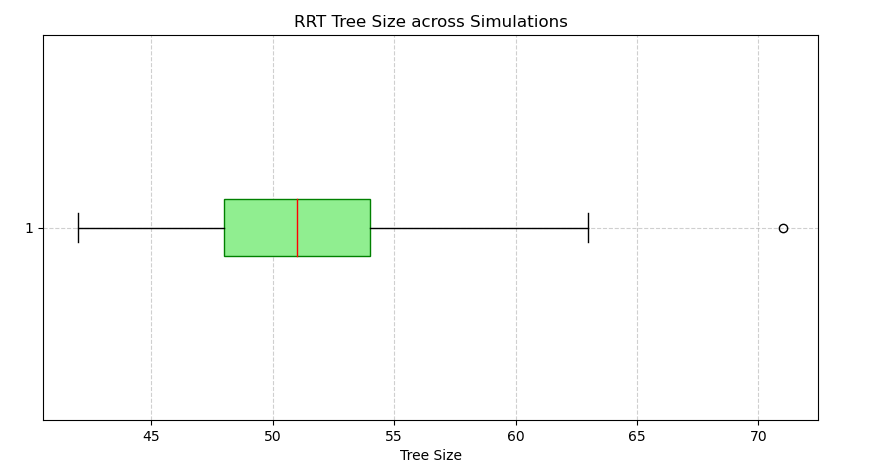
\includegraphics[width=0.7\textwidth]{1c2size.png} 
    \caption{Box plot for \(m = 2\) tree sizes over 100 iterations.}
    \label{fig:ic2size}
\end{figure}

\subsection*{(d) Repeat parts (b) and (c) for all \(m = 3, 4, 5, 6\)
Incrementally add agents from the list in logical order (i.e., \( m = 3 \) uses agents 1, 2, and 3, etc.). Show your results for every benchmark using boxplots. Save the data separately for future use.
}

\begin{figure}[H]
    \centering
    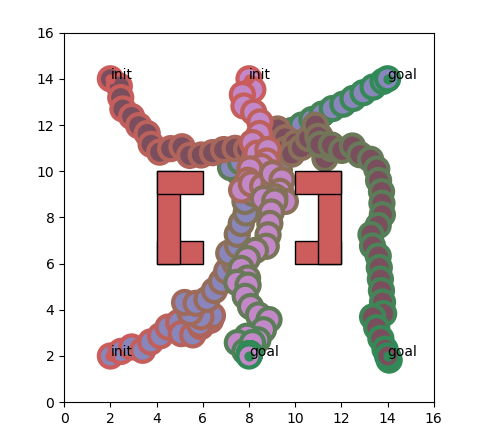
\includegraphics[width=0.7\textwidth]{1b3plot.png} 
    \caption{Solution plot for \(m = 3\) with agents reaching their respective goals.}
    \label{fig:1b3plot}
\end{figure}

\begin{figure}[H]
    \centering
    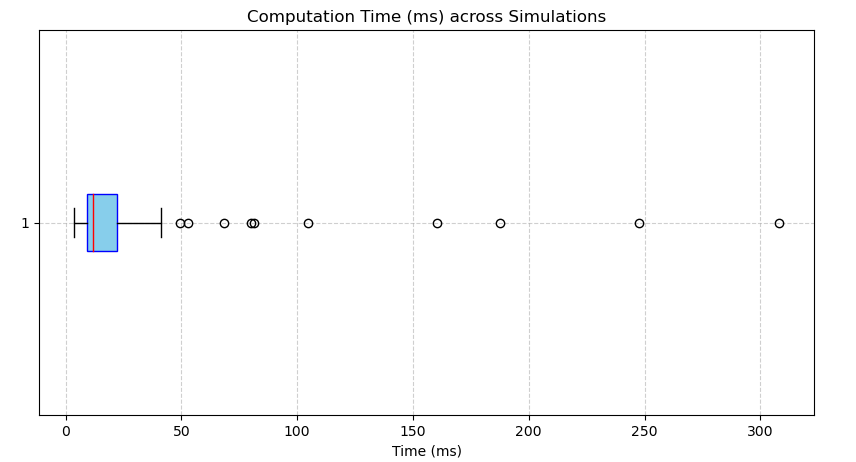
\includegraphics[width=0.7\textwidth]{1c3time.png} 
    \caption{Box plot for \(m = 3\) times over 100 iterations.}
    \label{fig:ic3time}
\end{figure}

\begin{figure}[H]
    \centering
    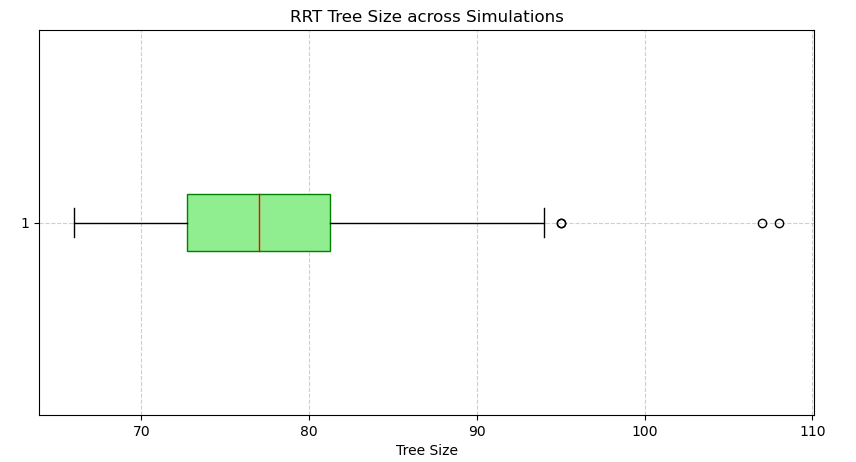
\includegraphics[width=0.7\textwidth]{1c3size.png} 
    \caption{Box plot for \(m = 3\) tree sizes over 100 iterations.}
    \label{fig:ic3size}
\end{figure}

\begin{figure}[H]
    \centering
    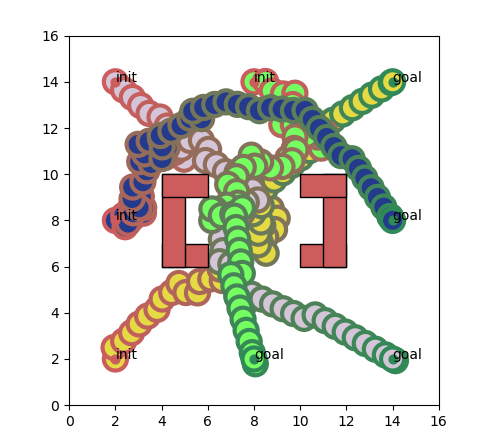
\includegraphics[width=0.7\textwidth]{1b4plot.png} 
    \caption{Solution plot for \(m = 4\) with agents reaching their respective goals.}
    \label{fig:1b4plot}
\end{figure}

\begin{figure}[H]
    \centering
    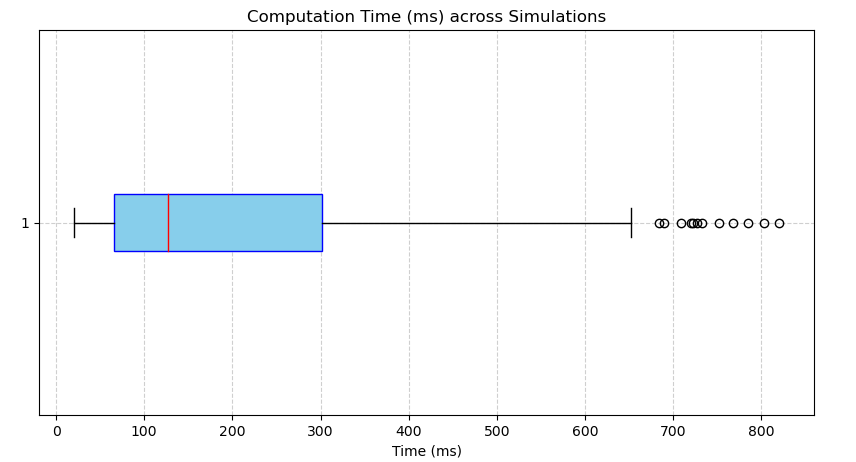
\includegraphics[width=0.7\textwidth]{1c4time.png} 
    \caption{Box plot for \(m = 4\) times over 100 iterations.}
    \label{fig:ic4time}
\end{figure}

\begin{figure}[H]
    \centering
    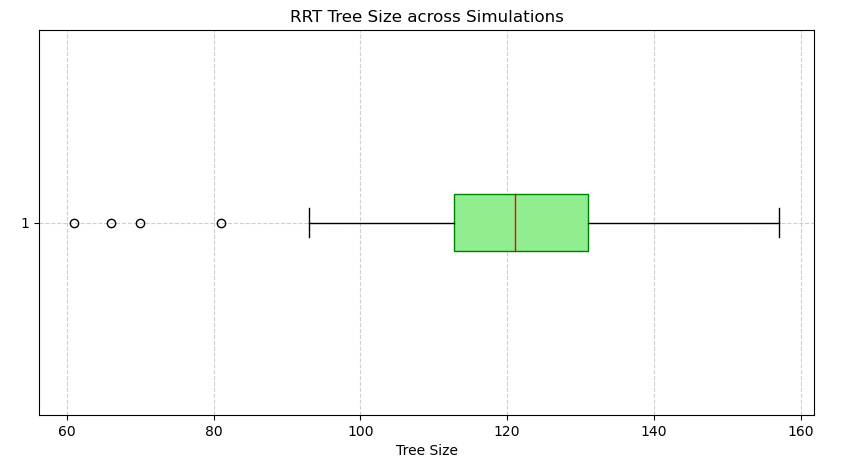
\includegraphics[width=0.7\textwidth]{1c4size.png} 
    \caption{Box plot for \(m = 4\) tree sizes over 100 iterations.}
    \label{fig:ic4size}
\end{figure}

\begin{figure}[H]
    \centering
    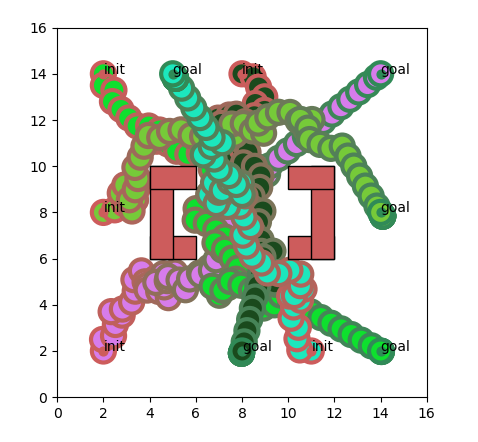
\includegraphics[width=0.7\textwidth]{1b5plot.png} 
    \caption{Solution plot for \(m = 5\) with agents reaching their respective goals.}
    \label{fig:1b5plot}
\end{figure}

\begin{figure}[H]
    \centering
    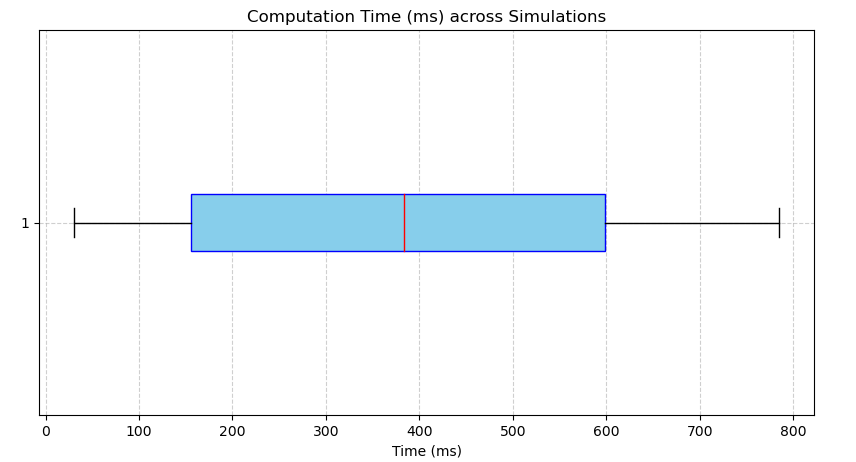
\includegraphics[width=0.7\textwidth]{1c5time.png} 
    \caption{Box plot for \(m = 5\) times over 100 iterations.}
    \label{fig:ic5time}
\end{figure}

\begin{figure}[H]
    \centering
    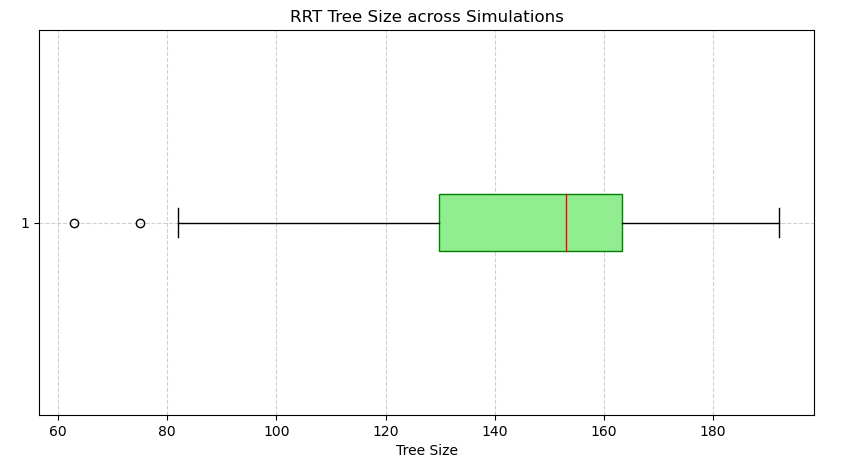
\includegraphics[width=0.7\textwidth]{1c5size.png} 
    \caption{Box plot for \(m = 5\) tree sizes over 100 iterations.}
    \label{fig:ic5size}
\end{figure}

\begin{figure}[H]
    \centering
    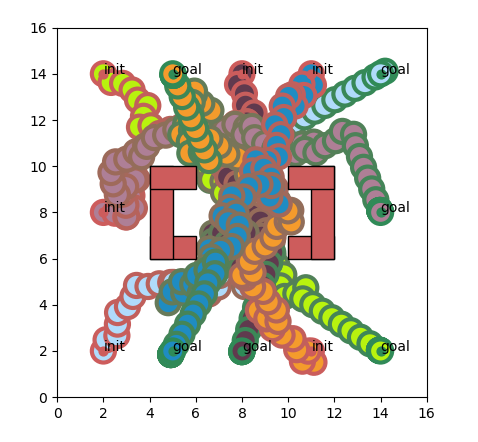
\includegraphics[width=0.7\textwidth]{1b6plot.png} 
    \caption{Solution plot for \(m = 6\) with agents reaching their respective goals.}
    \label{fig:1b6plot}
\end{figure}

\begin{figure}[H]
    \centering
    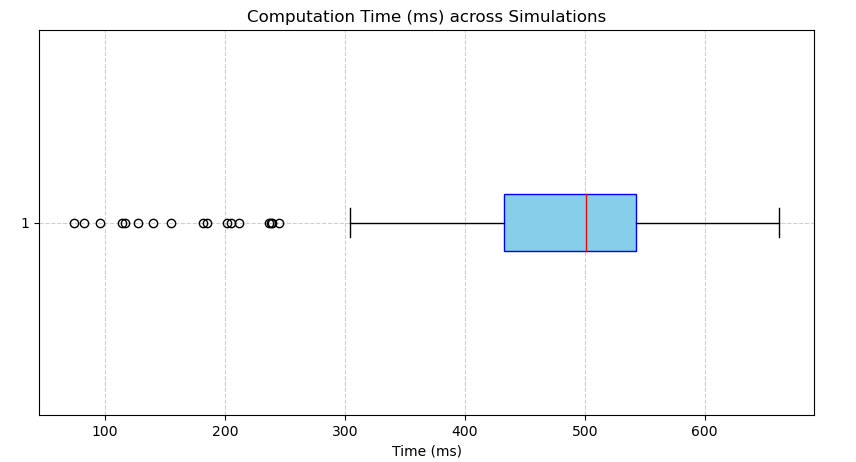
\includegraphics[width=0.7\textwidth]{1c6time.png} 
    \caption{Box plot for \(m = 6\) times over 100 iterations.}
    \label{fig:ic6time}
\end{figure}

\begin{figure}[H]
    \centering
    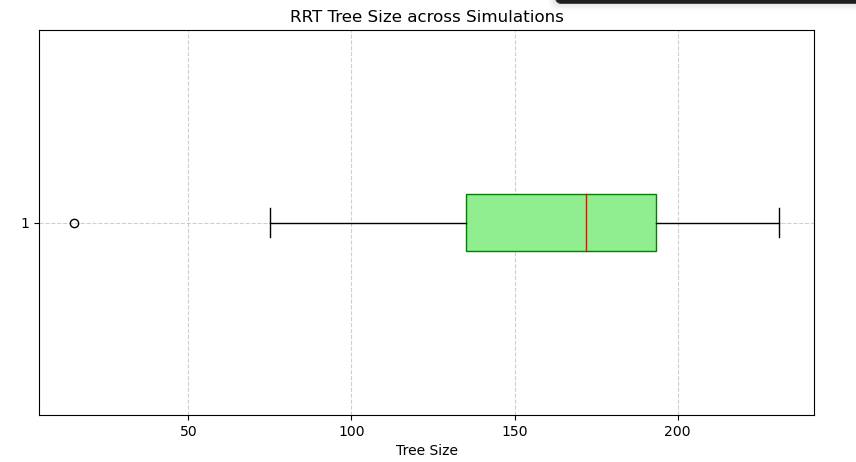
\includegraphics[width=0.7\textwidth]{1c6size.png} 
    \caption{Box plot for \(m = 6\) tree sizes over 100 iterations.}
    \label{fig:ic6size}
\end{figure}

\subsection*{(e)
Compute the average computation time and average size of tree over the 100 runs for each benchmark in (c) and (d). Use the 6 average computation times (1 for every value of $m$) and 6 average tree sizes to produce two plots:
\begin{itemize}
    \item An average computation time (y-axis) vs. number of agents $m$ (x-axis).
    \item An average size of tree (y-axis) vs. number of agents $m$ (x-axis).
\end{itemize}
Comment on what these plots tell us about increasing the number of agents.
}

\begin{figure}[H]
    \centering
    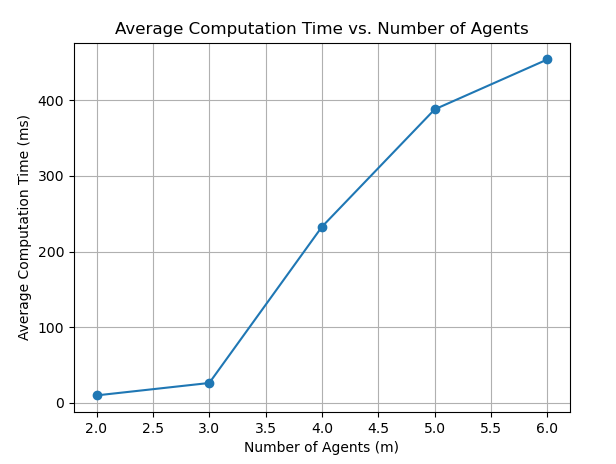
\includegraphics[width=0.7\textwidth]{1etime.png} 
    \caption{Average time for different m number of agents over 100 iterations.}
    \label{fig:ietime}
\end{figure}

\begin{figure}[H]
    \centering
    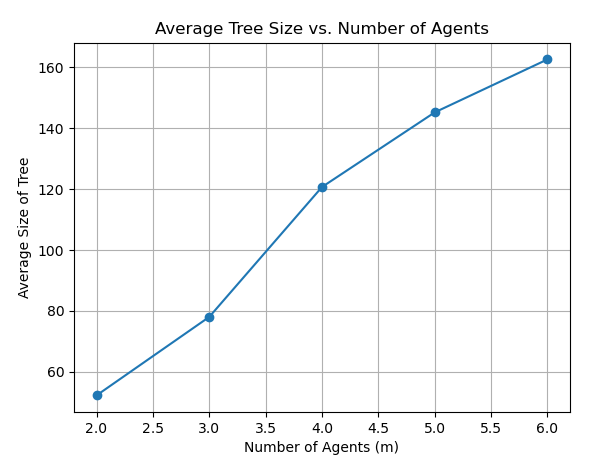
\includegraphics[width=0.7\textwidth]{1esize.png} 
    \caption{Average tree size for different m number of agents over 100 iterations.}
    \label{fig:iesize}
\end{figure}

\begin{itemize}
    \item \textbf{Average Tree Size vs. Number of Agents}: The size of the tree increases as the number of agents \( m \) grows. This can be attributed to the fact that with more agents, there are more potential paths to explore to avoid collisions and reach each agent's goal configuration. Consequently, the search space grows exponentially, leading to a larger tree.

    \item \textbf{Average Computation Time vs. Number of Agents}: The computation time also increases as the number of agents grows. This is expected, as managing more agents requires additional computations for collision checking, path planning, and overall coordination. The increased complexity in multi-agent planning results in a steep rise in computation time.
\end{itemize}

In conclusion, both the tree size and computation time exhibit near-exponential growth with respect to the number of agents. This behavior highlights the scalability challenge in multi-agent RRT-based planning methods: as the number of agents increases, the required computational resources and time to find feasible paths rise substantially. This trend suggests that for larger numbers of agents, optimized or alternative methods may be necessary to maintain feasible computation times.


\end{document}
